\chapter{Background}

\section{Basic Definitions}

In this section we provide some definitions that will be used throughout the thesis.

\begin{definition}[Multiset]
Let $U$ be an arbitrary set. A multiset over U is a mapping \newline $m : U \rightarrow N$.
The multiplicity of an element $u$ in $m$ is given by the natural number $m(s)$.
\end{definition}

\begin{definition}[Alphabet]
An alphabet is a finite nonempty set of abstract symbols. Given an alphabet $V$, we denote by $V^*$
the sets of all finite strings of elements in $V$, including the empty string $\lambda$.
Every string $v \in V$ describes a multiset over $V$.
\end{definition}


\section{P Systems}

We start from the most basic definition of a P system.

\begin{definition}[P system]
A P system (of degree $d$, with $d \geq 1$) is a tuple
\[ \Pi = (V,\mu,w^0_1,...,w^0_d,R_1,...,R_d)\]
where:
\begin{enumerate}
  \item $V$ is an alphabet; its elements are called objects;
  \item $\mu$ is a membrane structure consisting of $d$ membranes (labeled with $1,2,...,d$);
  \item $w^0_1, 1 \leq i \leq d$, are strings from $V^*$ representing multisets over $V$ associated
  with the regions $1,2,...,d$ of $\mu$;
  \item $R_i, 1 \leq i \leq d$, are finite sets of evolution rules over $V$ associated 
  with the regions $1,2,...,d$ of $\mu$; these evolution rules are of the form $u \rightarrow v$,
  where $u$ and $v$ are strings from $V*$;
\end{enumerate}
A configuration of $\Pi$ is a tuple $C=(w_1,...,w_d)$ of multisets of objects, and 
$C_0=(w^0_1,...,w^0_d)$ is the initial configuration.
\end{definition}

For the sake of simplicity, in what follows, we consider the flat (or elementary) P system, that is a P system of degree one.
Actually, according to \cite{agrigoroaiei2010flattening}, any P system can be flattened to a system with only one membrane.

\begin{definition}[Flat P system]
A flat P system is a P system of degree one
\[ \Pi = (V,\mu,w^0,R) \]

Given the fact that we're working with a one degree system we removed the subscript from $w$ and $R$. 
A configuration of $\Pi$ is a singleton $C=(w)=w$ of a multiset of objects, and 
$C_0=(w^0)=w^0$ is the initial configuration.
\end{definition}

Let's see an example of a flat P system.

\begin{figure}[h]
\centering

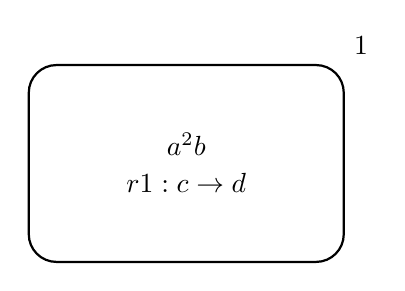
\begin{tikzpicture}
    \draw[thick, rounded corners=10pt] (0, 0) rectangle (4, 2.5) node[above right] {1};
    
    \node at (2, 1.5) {$a^2b$};
    \node at (2,1) (rule) {$r1: c \rightarrow d$};
\end{tikzpicture}

\caption{}
\label{}
\end{figure}

From now on when we talk about P systems we are talking of flat P systems.

\subsection{Synchronized P systems}

Here we extend the latter definition of a flat P System with the concept of synchronization. 

\begin{definition}[Synchronized P system]
A synchronized P system of degree 1 is a tuple

\[ \Pi = (V,\mu,w^0,(R,\rho)) \]

where:
\begin{enumerate}
  \item $\rho$ is a partial relation defined over the set $R$ of rules specifying
  the synchronization relation over the rules;
  $\rho$ is irreflexive, asymmetric and transitive;
\end{enumerate}
\end{definition}

Let's try to understand better what syncronization means:
let $(r1,r2) \in \rho$; if $r1$ is executed at least one time, then also
$r2$ has to be executed at least one time during this step, and vice versa; if that is not possible neither of them will be executed during the current step.

We use the following notation to describe an instance of $\rho$: 
$\rho=((r1 \otimes r2),(r3 \otimes r4 \otimes r5))$.
This means that $r_1$ can be executed only and only if $r_2$ can be executed at least one time;
in addition, $r_1$ it's executed at least one time only and only if also $r_2$ it's executed at least one time.
Let's see an example to grasp the concept...

\begin{definition}[synchronization rule]
\label{def:sync_rule}
We define a synchronization rule $r_s$ as a set of rules defined by a tuple in $\rho$.
\end{definition}

So given the previous example $(r1 \otimes r2) \in \rho$ then $r_s=\{r1,r2\}$.

\section{Petri Net}

Here we define in a formal way what a Petri Net is.

\subsection{Petri Nets with Inhibitor Arcs}

Here we extend the latter definition of a Petri Net with the concept of inhibitor arcs.